The music filter layer concicts if the Pre-Amp and three music filters which are responsible for amplifyind the music sound and filtering the frequencies of the filter.

\subsection{Pre-Amp}
This Pre-Amp is responsible for amplifying the sound signal that is passed on from the raspberry pi in order to be big enough to be picked up by the filters.

\begin{figure}[h!]
	\centering
 	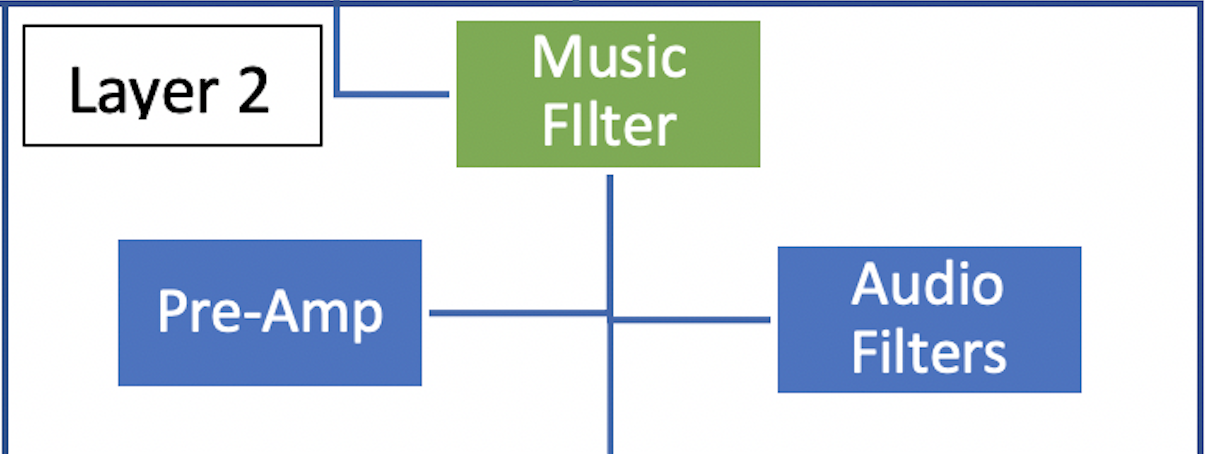
\includegraphics[width=0.60\textwidth]{images/subsystem2}
 \caption{Subsystem 2 Diagram}
\end{figure}

\subsubsection{Assumptions}
The pre-amp receives input from the raspberry pi and will send the output signal to the filters .

\subsubsection{Responsibilities}
The pre-amp's responsibility is to amplify the signal that comes from the raspberry pi, so that it will be big enought to be picked up by the filters and audio amplifier 

\subsubsection{Subsystem Interfaces}
The raspberry pi sends a signal input to the pre-amp

\begin {table}[H]
\caption {Subsystem interfaces} 
\begin{center}
    \begin{tabular}{ | p{1cm} | p{6cm} | p{3cm} | p{3cm} |}
    \hline
    ID & Description & Inputs & Outputs \\ \hline
    \#1 & Pre-amp & \pbox{3cm}{audio signal} & \pbox{3cm}{amplified audio signal}  \\ \hline
    \end{tabular}
\end{center}
\end{table}

\subsection{Audio Filters}
The audio filters are three: Lowpass, Bandpass and Highpass filters that filter the low, high and mid frequencies of the signal that the pre amp outputs.

\begin{figure}[h!]
	\centering
 	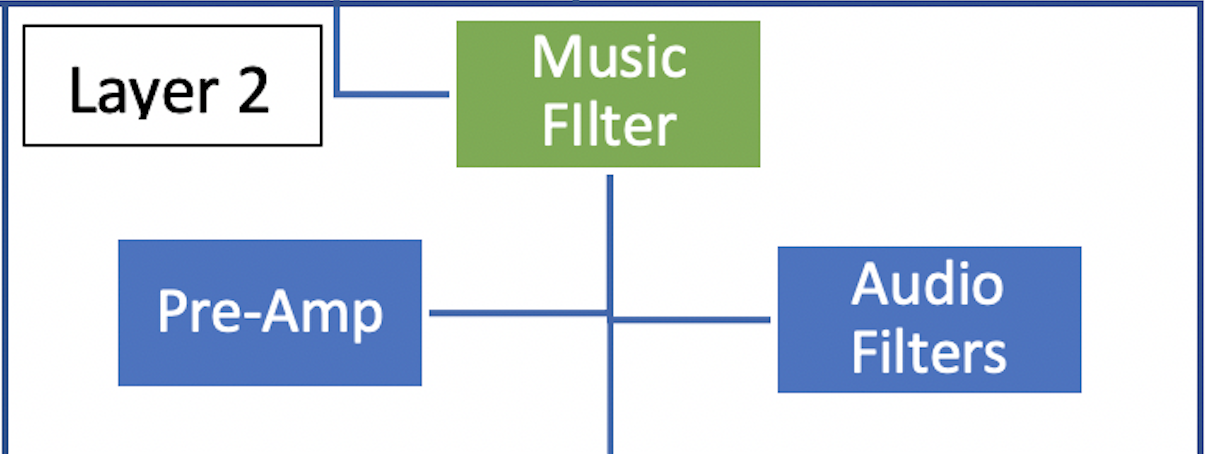
\includegraphics[width=0.60\textwidth]{images/subsystem2}
 \caption{Lowpass, Highpass and Bandpass filters}
\end{figure}

\subsubsection{Assumptions}
The signal from the pre-amp will be amplified enought o be picked up by the filters.

\subsubsection{Responsibilities}
The output signal from the pre-amp are passed through the three filters to be divided into low frequency, high frequncy and mid frequency signals

\subsubsection{Subsystem Interfaces}
The input for each of the filters will be the output signal from the pre-amp and the signal will be filtered to provide either the low, mid , amd high frequency signals or sounds which will then be sent to the audio amplifier

\begin {table}[H]
\caption {Subsystem interfaces} 
\begin{center}
    \begin{tabular}{ | p{1cm} | p{6cm} | p{3cm} | p{3cm} |}
    \hline
    ID & Description & Inputs & Outputs \\ \hline
    \#2 & Lowpass filter & \pbox{3cm}{input from the output signal of the pre-amp} & \pbox{3cm}{low frequancy signal}  \\ \hline
    \#3 & Highpass filter & \pbox{3cm}{input from the output signal of the preamp } & \pbox{3cm}{high frequency signal}  \\ \hline
    \#4 & Bandpass filter & \pbox{3cm}{input from the output signal of the preamp } & \pbox{3cm}{mid frequency signal}  \\ \hline
    \end{tabular}
\end{center}
\end{table}

